\providecommand{\qcOne}{\mathbf{1}}   %
\providecommand{\qcor}[1]{\ulcorner#1\urcorner}   %

\section{伴随的\trUniversalProperty}\label{sec:universal-property-of-adjunctions}

一对对立的\trFunctor{}之间的\trAdjunction{}，同样可以由二者作为%
\trCommaInfinityCategory{}的左表示与右表示之间的一个「转置等价」来编码。

\begin{proposition}[作为\trFiberedEquivalence{}的\trAdjunction]\label{prop:adjunction-as-fibered-equivalence}
一对对立的\trFunctor{} $u\colon A\to B$ 与 $f\colon B\to A$ 构成一个%
\trAdjunction{} $f\dashv u$，当且仅当
$\mathrm{Hom}_A(f,A)\simeq_{A\times B}\mathrm{Hom}_B(B,u)$。
\end{proposition}

这是定理 3.5.8 的一个特例，故本无需进一步论证；但我们仍然给出一个简短的%
证明，以温习 3.5 节中证明过的那些结果。

\begin{proof}
若 $f\dashv u$，则由引理 2.3.7，其\trCounit{}
$\epsilon\colon fu\Rightarrow\mathrm{id}_A$ 定义了一个绝对右\trLifting{}图。
据定理 3.5.8，左侧的粘贴复合
\begin{center}
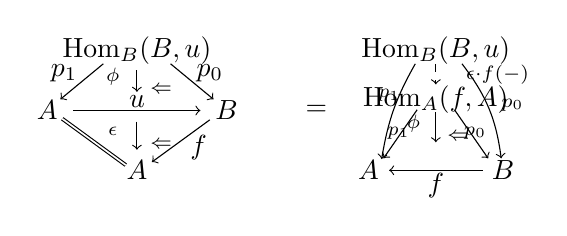
\begin{tikzpicture}[x=1.35em,y=1.35em]
  \node (H1) at (1.8,3.2) {$\mathrm{Hom}_B(B,u)$};
  \node (A2) at (-0.6,1.6) {$A$};
  \node (B2) at (4.2,1.6) {$B$};
  \node (A3) at (1.8,0) {$A$};
  \draw[->] (0.9,2.85) -- (-0.25,1.9);
  \node at (-0.15,2.6) {$p_1$};
  \draw[->] (2.7,2.85) -- (3.85,1.9);
  \node at (3.75,2.6) {$p_0$};
  \draw[->] (1.8,2.68) -- (1.8,2.1);
  \node at (1.15,2.5) {$\scriptstyle\phi$};
  \node at (2.45,2.15) {$\scriptstyle\Leftarrow$};
  \draw[->] (0.1,1.6) -- (3.5,1.6);
  \node at (1.8,1.85) {$u$};
  \draw[double] (-0.2,1.38) -- (1.5,0.14);
  \draw[->] (3.75,1.35) -- (2.2,0.22);
  \node at (3.45,0.6) {$f$};
  \draw[->] (1.8,1.3) -- (1.8,0.55);
  \node at (1.15,1.05) {$\scriptstyle\epsilon$};
  \node at (2.45,0.68) {$\scriptstyle\Leftarrow$};
  \node at (6.6,1.6) {$=$};
  \node (H2) at (9.8,3.2) {$\mathrm{Hom}_B(B,u)$};
  \node (M2) at (9.8,1.9) {$\mathrm{Hom}_A(f,A)$};
  \node (A4) at (8.0,0) {$A$};
  \node (B4) at (11.6,0) {$B$};
  \draw[->,dashed] (9.8,2.85) -- (9.8,2.3);
  \node at (11.45,2.55) {$\scriptstyle\qcor{\epsilon\cdot f(-)}$};
  \draw[->] (9.25,2.85) to[bend right=10] (8.35,0.3);
  \node at (8.55,2.0) {$\scriptstyle p_1$};
  \draw[->] (10.5,2.85) to[bend left=15] (11.55,0.32);
  \node at (11.85,1.75) {$\scriptstyle p_0$};
  \draw[->] (9.3,1.62) -- (8.4,0.32);
  \node at (8.8,1.0) {$\scriptstyle p_1$};
  \draw[->] (10.3,1.62) -- (11.2,0.32);
  \node at (10.85,1.0) {$\scriptstyle p_0$};
  \draw[->] (9.8,1.55) -- (9.8,0.75);
  \node at (9.2,1.25) {$\scriptstyle\phi$};
  \node at (10.4,0.9) {$\scriptstyle\Leftarrow$};
  \draw[->] (11.05,0) -- (8.55,0);
  \node at (9.8,-0.42) {$f$};
\end{tikzpicture}
\end{center}
所诱导的\trFunctor{}定义了一个\trFiberedEquivalence{}
$\mathrm{Hom}_B(B,u)\simeq_{A\times B}\mathrm{Hom}_A(f,A)$。我们把这一结果%
诠释为如下断言：在\trAdjunction{} $f\dashv u$ 存在时，$u$ 之上的右%
\trCommaCone{}经转置即定义 $f$ 之上的左\trCommaCone{}。%
\footnote{如果愿意，也可以对由\trUnit{}所呈现的绝对左\trLifting{}图应用%
定理 3.5.8 的对偶形式，构造出一个逆\trEquivalence。}

反之，从一个\trFiberedEquivalence{}
$\mathrm{Hom}_B(B,u)\simeq_{A\times B}\mathrm{Hom}_A(f,A)$ 出发，定理 3.5.8
告诉我们：可以提取出一个 2-\trCell，它定义了绝对右\trLifting{}图
\begin{center}
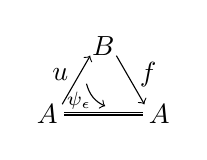
\begin{tikzpicture}[x=1.35em,y=1.35em]
  \node (Bl) at (1.5,1.8) {$B$};
  \node (Al) at (0,0) {$A$};
  \node (Ar) at (3.0,0) {$A$};
  \draw[double] (0.45,0) -- (2.55,0);
  \draw[->] (0.4,0.25) -- (1.15,1.55);
  \node at (0.35,1.05) {$u$};
  \draw[->] (1.85,1.55) -- (2.6,0.25);
  \node at (2.7,1.05) {$f$};
  \draw[->] (1.05,0.8) to[bend right=25] (1.55,0.2);
  \node at (0.85,0.35) {$\scriptstyle\psi_{\epsilon}$};
\end{tikzpicture}
\end{center}
而由引理 2.3.7，它进而定义了\trAdjunction{} $f\dashv u$ 的\trCounit{}。
\end{proof}

\begin{observation}[转置等价]\label{obs:transposing-equivalence}
为论证把诱导\trFunctor
\[
\qcor{\epsilon\cdot f(-)}\colon \mathrm{Hom}_B(B,u)\twoheadrightarrow
\mathrm{Hom}_A(f,A)
\]
称作\textbf{转置等价}（transposing equivalence）的做法，回顾如下事实：
一个 2-\trCell{} $\chi\colon b\Rightarrow ua$ 沿\trAdjunction{} $f\dashv u$
的转置，由下方左侧的粘贴图计算：
\begin{center}
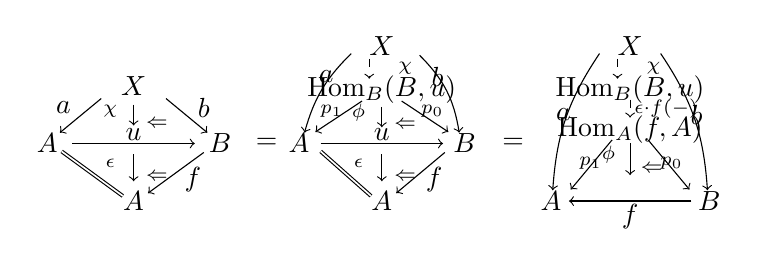
\begin{tikzpicture}[x=1.3em,y=1.3em]
  \node at (1.8,3.2) {$X$};
  \node (LA2) at (-0.6,1.6) {$A$};
  \node (LB2) at (4.2,1.6) {$B$};
  \node (LA3) at (1.8,0) {$A$};
  \draw[->] (0.9,2.85) -- (-0.25,1.9);
  \node at (-0.15,2.6) {$a$};
  \draw[->] (2.7,2.85) -- (3.85,1.9);
  \node at (3.75,2.6) {$b$};
  \draw[->] (1.8,2.68) -- (1.8,2.1);
  \node at (1.15,2.5) {$\scriptstyle\chi$};
  \node at (2.45,2.15) {$\scriptstyle\Leftarrow$};
  \draw[->] (0.1,1.6) -- (3.5,1.6);
  \node at (1.8,1.85) {$u$};
  \draw[double] (-0.2,1.38) -- (1.5,0.14);
  \draw[->] (3.75,1.35) -- (2.2,0.22);
  \node at (3.45,0.6) {$f$};
  \draw[->] (1.8,1.3) -- (1.8,0.55);
  \node at (1.15,1.05) {$\scriptstyle\epsilon$};
  \node at (2.45,0.68) {$\scriptstyle\Leftarrow$};
  \node at (5.5,1.6) {$=$};
  \node at (8.7,4.3) {$X$};
  \draw[->,dashed] (8.35,3.95) -- (8.35,3.4);
  \node at (9.35,3.68) {$\scriptstyle\qcor{\chi}$};
  \node at (8.7,3.1) {$\mathrm{Hom}_B(B,u)$};
  \draw[->] (7.85,4.1) to[bend right=15] (6.55,1.9);
  \node at (7.15,3.45) {$a$};
  \draw[->] (9.75,4.05) to[bend left=18] (10.85,1.9);
  \node at (10.25,3.45) {$b$};
  \draw[->] (8.15,2.78) -- (6.85,1.92);
  \node at (7.3,2.5) {$\scriptstyle p_1$};
  \draw[->] (9.25,2.78) -- (10.55,1.92);
  \node at (10.1,2.5) {$\scriptstyle p_0$};
  \draw[->] (8.7,2.62) -- (8.7,2.05);
  \node at (8.05,2.45) {$\scriptstyle\phi$};
  \node at (9.35,2.12) {$\scriptstyle\Leftarrow$};
  \draw[->] (7.0,1.6) -- (10.4,1.6);
  \node at (8.7,1.85) {$u$};
  \draw[double] (7.0,1.38) -- (8.4,0.14);
  \draw[->] (10.45,1.35) -- (9.1,0.22);
  \node at (10.15,0.6) {$f$};
  \draw[->] (8.7,1.3) -- (8.7,0.55);
  \node at (8.05,1.05) {$\scriptstyle\epsilon$};
  \node at (9.35,0.68) {$\scriptstyle\Leftarrow$};
  \node at (6.4,1.6) {$A$};
  \node at (11.0,1.6) {$B$};
  \node at (8.7,0) {$A$};
  \node at (12.35,1.6) {$=$};
  \node at (15.6,4.3) {$X$};
  \draw[->,dashed] (15.25,3.95) -- (15.25,3.4);
  \node at (16.25,3.68) {$\scriptstyle\qcor{\chi}$};
  \node at (15.6,3.1) {$\mathrm{Hom}_B(B,u)$};
  \draw[->] (14.75,4.1) to[bend right=15] (13.45,0.3);
  \node at (13.75,2.4) {$a$};
  \draw[->] (16.45,4.1) to[bend left=15] (17.75,0.3);
  \node at (17.45,2.4) {$b$};
  \draw[->,dashed] (15.6,2.82) -- (15.6,2.32);
  \node at (16.6,2.58) {$\scriptstyle\qcor{\epsilon\cdot f(-)}$};
  \node at (15.6,2.0) {$\mathrm{Hom}_A(f,A)$};
  \draw[->] (15.1,1.7) -- (13.95,0.32);
  \node at (14.5,1.05) {$\scriptstyle p_1$};
  \draw[->] (16.1,1.7) -- (17.25,0.32);
  \node at (16.75,1.05) {$\scriptstyle p_0$};
  \draw[->] (15.6,1.62) -- (15.6,0.72);
  \node at (15.0,1.28) {$\scriptstyle\phi$};
  \node at (16.2,0.9) {$\scriptstyle\Leftarrow$};
  \node at (13.4,0) {$A$};
  \node at (17.8,0) {$B$};
  \draw[->] (17.3,0) -- (13.9,0);
  \node at (15.6,-0.42) {$f$};
\end{tikzpicture}
\end{center}
由 $u$ 之上的右\trCommaCone{}的弱\trUniversalProperty，2-\trCell{} $\chi$
由诱导\trFunctor{} $\qcor{\chi}\colon X\to\mathrm{Hom}_B(B,u)$ 表示；
$\qcor{\chi}$ 再与转置等价复合，便定义了\trFunctor{}
$\qcor{\epsilon\cdot f(\chi)}\colon X\to\mathrm{Hom}_A(f,A)$——由自右至左的%
粘贴图等式，它所表示的正是 $\chi$ 的转置。这一观察也正当化了我们的记号：
我们为该\trFiberedEquivalence{}取名为 $\qcor{\epsilon\cdot f(-)}$，其名得自%
伴随转置的公式。
\end{observation}

\begin{corollary}\label{cor:adjunction-generalized-elements}
一对对立的\trFunctor{} $u\colon A\to B$ 与 $f\colon B\to A$ 构成一个%
\trAdjunction{} $f\dashv u$，当且仅当对任意一对\trGeneralizedElement{}
$a\colon X\to A$ 与 $b\colon Y\to B$，存在一个\trEquivalence{}
$\mathrm{Hom}_A(fb,a)\simeq_{X\times Y}\mathrm{Hom}_B(b,ua)$。
\end{corollary}

\begin{proof}
当 $f\dashv u$ 时，沿 $a\times b\colon X\times Y\to A\times B$ 的\trPullback{}%
定义了一个\trCosmologicalFunctor，它把\cref{prop:adjunction-as-fibered-equivalence}的%
\trEquivalence{} $\mathrm{Hom}_A(f,A)\simeq_{A\times B}\mathrm{Hom}_B(B,u)$
搬运为\trEquivalence{}
$\mathrm{Hom}_A(fb,a)\simeq_{X\times Y}\mathrm{Hom}_B(b,ua)$。反之，取%
\trGeneralizedElement{}为恒同\trFunctor{} $\mathrm{id}_A$ 与 $\mathrm{id}_B$
的特殊情形，即证得逆命题。
\end{proof}

\begin{remark}\label{rem:internal-mapping-spaces}
特别地，\cref{prop:adjunction-as-fibered-equivalence}的\trEquivalence{}经%
\trPullback{}定义了诸内部\trMappingSpace{}的一个\trEquivalence；内部%
\trMappingSpace{}由定义 3.4.9 引入。
在推论 12.2.15 中我们将看到：在一个由 $(\infty,1)$-\trCategory{}构成的%
\trInfinityCosmos{}中，一个\trNaturalTransformation{}
$\epsilon\colon fu\Rightarrow\mathrm{id}_A$ 定义某个\trAdjunction{}的%
\trCounit，当且仅当映射
$\qcor{\epsilon\cdot f(-)}\colon\mathrm{Hom}_B(B,u)\to\mathrm{Hom}_A(f,A)$
对任意一对元素 $a\colon\qcOne\to A$ 与 $b\colon\qcOne\to B$ 都定义内部%
\trMappingSpace{}的\trEquivalence{}
$\mathrm{Hom}_B(b,ua)\simeq\mathrm{Hom}_A(fb,a)$。
\end{remark}

\trCommaInfinityCategory{}也为表达\trUnit{}与\trCounit{}变换的%
\trUniversalProperty{}提供了一种载体。

\begin{proposition}[单位与余单位的泛性质]\label{prop:universal-property-units-counits}
考虑\trAdjunction
\begin{center}
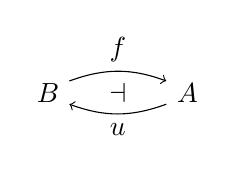
\begin{tikzpicture}[x=1.4em,y=1.4em]
  \node (B1) at (0,0) {$B$};
  \node (A1) at (3.6,0) {$A$};
  \draw[->] (0.55,0.3) to[bend left=20] node[above]{$f$} (3.05,0.3);
  \node at (1.8,0) {$\dashv$};
  \draw[->] (3.05,-0.3) to[bend left=20] node[below]{$u$} (0.55,-0.3);
\end{tikzpicture}
\end{center}
配有\trUnit{} $\eta\colon\mathrm{id}_B\Rightarrow uf$ 与\trCounit{}
$\epsilon\colon fu\Rightarrow\mathrm{id}_A$。则对每个元素
$a\colon\qcOne\to A$，分量 $\epsilon_a$ 定义了 $\mathrm{Hom}_A(f,a)$ 的一个%
\trTerminal{}元素，而对每个元素 $b\colon\qcOne\to B$，分量 $\eta_b$ 定义了
$\mathrm{Hom}_B(b,u)$ 的一个\trInitial{}元素。
\end{proposition}

\begin{proof}
\cref{prop:adjunction-as-fibered-equivalence}的\trFiberedEquivalence{}
$\mathrm{Hom}_A(f,A)\simeq_{A\times B}\mathrm{Hom}_B(B,u)$
依\cref{cor:adjunction-generalized-elements}经\trPullback{}定义了下列诸%
\trEquivalence：
\[
\mathrm{Hom}_A(f,a)\simeq_{B}\mathrm{Hom}_B(B,ua)
\qquad\text{与}\qquad
\mathrm{Hom}_A(fb,A)\simeq_{A}\mathrm{Hom}_B(b,u)
\]
由推论 3.5.10，$\mathrm{id}_{ua}$ 在 $\mathrm{Hom}_B(B,ua)$ 中诱导出一个%
\trTerminal{}元素，而由引理 2.2.7，其沿\trEquivalence{}
$\mathrm{Hom}_B(B,ua)\simeq\mathrm{Hom}_A(f,a)$ 的像仍是\trTerminal{}元素。
由\cref{obs:transposing-equivalence}，该元素表示那个转置后的 2-\trCell：即%
\trCounit{} $\epsilon$ 在元素 $a$ 处的分量。
\end{proof}

\cref{prop:universal-property-units-counits}所捕捉的\trUnit{}与\trCounit{}%
分量之\trUniversalProperty{}给出了伴随函子定理背后的主要思想。
在一个由 $(\infty,1)$-\trCategory{}构成的\trInfinityCosmos{}中，一个%
\trFunctor{} $f\colon B\to A$ 容许一个\trRightAdjoint，恰好当对每个元素
$a\colon\qcOne\to A$，\trInfinityCategory{} $\mathrm{Hom}_A(f,a)$ 容许一个%
\trTerminal{}元素（见推论 12.2.7）。
\footnote{回顾例 2.3.11：一个\trTerminal{}元素是恒同\trFunctor{}的一个%
\trColimit。Freyd 的一般伴随函子定理与特殊伴随函子定理中所部署的技术性条件，
正是为了把这个大\trColimit{}约减为小\trColimit{}并保证其存在性（这些结果的一个%
1-范畴式表述见 \cite[\S 4.6]{bib104}）。类似的定理已由 Nguyen、Raptis 与
Schrade 在 $(\infty,1)$-范畴语境中证明 \cite{bib88}。}
该\trTerminal{}元素在定义域投影函子
$p_0\colon\mathrm{Hom}_A(f,a)\twoheadrightarrow B$ 之下的像定义了元素
$ua\colon\qcOne\to B$，而\trCommaCone{}则定义了\trCounit{}在 $a$ 处的分量。
\trCounit{}分量的\trUniversalProperty{}随后被用于把元素上的这一映射扩充为
一个\trFunctor{} $u\colon A\to B$。

一个在一般\trInfinityCosmos{}中亦真的类似结果可以这样得到：把量词「对每个%
元素 $a\colon\qcOne\to A$」换成「对每个\trGeneralizedElement{}
$a\colon X\to A$」，此时「\trTerminal{}元素」的含义应当增强为「$X$ 之上的%
\trTerminal{}元素」（见定义 3.6.8）。
由于每个\trGeneralizedElement{}都经由那个泛\trGeneralizedElement{}——即 $A$
处的恒同\trFunctor{}——分解，故只需证明：

\begin{proposition}\label{prop:adjoint-criterion-terminal-element}
一个\trFunctor{} $f\colon B\to A$ 容许一个\trRightAdjoint，当且仅当
$\mathrm{Hom}_A(f,A)$ 容许一个 $A$ 之上的\trTerminal{}元素。对偶地，
$f\colon B\to A$ 容许一个\trLeftAdjoint，当且仅当 $\mathrm{Hom}_A(A,f)$
容许一个 $A$ 之上的\trInitial{}元素。
\end{proposition}

\begin{proof}
由\cref{prop:adjunction-as-fibered-equivalence}，\trFunctor{}
$f\colon B\to A$ 容许一个\trRightAdjoint，当且仅当\trCommaInfinityCategory{}
$\mathrm{Hom}_A(f,A)$ 是右\trRepresentable；而据推论 3.6.10，此情形恰在
$\mathrm{Hom}_A(f,A)$ 容许一个 $A$ 之上的\trTerminal{}元素时成立。
\end{proof}

3.5–3.6 节的同一组成果均可特化为编码\trLimit{}与\trColimit{}之%
\trUniversalProperty{}的定理。在探究这些之前，我们先来构造一个\trDiagram{}%
之上或之下的\trInfinityCategoryOfCones{}。

\subsection*{练习}

\begin{exercise}[4.3.13]\label{ex:specialize-point-adjunctions}
将\cref{prop:adjunction-as-fibered-equivalence}特化到伴随
\begin{center}
\begin{tikzpicture}[x=1.4em,y=1.4em]
  \node (P1) at (0,0) {$\qcOne$};
  \node (QA1) at (3.4,0) {$A$};
  \draw[->] (0.5,0.3) to[bend left=20] node[above]{$i$} (2.9,0.3);
  \node at (1.7,0) {$\dashv$};
  \draw[->] (2.9,-0.3) to[bend left=20] node[below]{$!$} (0.5,-0.3);
  \node at (5.2,0) {与};
  \node (P2) at (7.0,0) {$\qcOne$};
  \node (QA2) at (10.4,0) {$A$};
  \draw[->] (9.9,0.3) to[bend right=20] node[above]{$!$} (7.5,0.3);
  \node at (8.7,0) {$\dashv$};
  \draw[->] (7.5,-0.3) to[bend right=20] node[below]{$t$} (9.9,-0.3);
\end{tikzpicture}
\end{center}
的情形，以发现\trInitial{}元素与\trTerminal{}元素的另一种刻画。
\end{exercise}

\begin{exercise}\label{ex:naturality-of-transposing-equivalence}
对于任意一对平行的、完全给定的\trAdjunction
\begin{center}
\begin{tikzpicture}[x=1.4em,y=1.4em]
  \node (B1) at (0,0) {$B$};
  \node (A1) at (3.6,0) {$A$};
  \draw[->] (0.55,0.3) to[bend left=20] node[above]{$f$} (3.05,0.3);
  \node at (1.8,0) {$\dashv$};
  \draw[->] (3.05,-0.3) to[bend left=20] node[below]{$u$} (0.55,-0.3);
  \node at (5.3,0) {与};
  \node (B2) at (7.0,0) {$B$};
  \node (A2) at (10.6,0) {$A$};
  \draw[->] (7.55,0.3) to[bend left=20] node[above]{$f'$} (10.05,0.3);
  \node at (8.8,0) {$\dashv$};
  \draw[->] (10.05,-0.3) to[bend left=20] node[below]{$u'$} (7.55,-0.3);
\end{tikzpicture}
\end{center}
前者配有\trUnit{} $\eta\colon\mathrm{id}_B\Rightarrow uf$ 与\trCounit{}
$\epsilon\colon fu\Rightarrow\mathrm{id}_A$，后者配有\trUnit{}
$\eta'\colon\mathrm{id}_B\Rightarrow u'f'$ 与\trCounit{}
$\epsilon'\colon f'u'\Rightarrow\mathrm{id}_A$；则在\trNaturalTransformation{}
$\alpha\colon f'\Rightarrow f$ 与 $\beta\colon u\Rightarrow u'$ 之间存在一个%
双射，此即\emph{\trMate}（mates correspondence）的一个特例（见定义 B.3.3）。
请论证：\cref{prop:adjunction-as-fibered-equivalence}的转置等价对于「以
2-\trCell{} $\alpha\colon f'\Rightarrow f$ 作预复合」以及「以其\trMate
$\beta\colon u\Rightarrow u'$ 作后复合」（见推论 3.5.11）都是自然的，
为此请证明：在下列诸\trFunctor{}之间存在 $A\times B$ 之上的一个纤维化自然%
同构：
\begin{center}
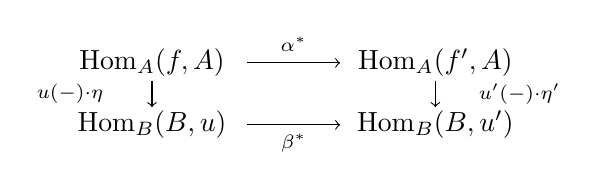
\begin{tikzpicture}[x=1.6em,y=1.6em]
  \node (TL) at (0,1.4) {$\mathrm{Hom}_A(f,A)$};
  \node (TR) at (6.4,1.4) {$\mathrm{Hom}_A(f',A)$};
  \node (BL) at (0,0) {$\mathrm{Hom}_B(B,u)$};
  \node (BR) at (6.4,0) {$\mathrm{Hom}_B(B,u')$};
  \draw[->] (2.15,1.4) -- (4.25,1.4);
  \node at (3.2,1.82) {$\scriptstyle\qcor{\alpha^{*}}$};
  \draw[->] (0,1.0) -- (0,0.4);
  \node at (-1.85,0.7) {$\scriptstyle\qcor{u(-)\cdot\eta}$};
  \draw[->] (6.4,1.0) -- (6.4,0.4);
  \node at (8.3,0.7) {$\scriptstyle\qcor{u'(-)\cdot\eta'}$};
  \draw[->] (2.15,0) -- (4.25,0);
  \node at (3.2,-0.42) {$\scriptstyle\qcor{\beta^{*}}$};
\end{tikzpicture}
\end{center}
\end{exercise}
